% Options for packages loaded elsewhere
\PassOptionsToPackage{unicode}{hyperref}
\PassOptionsToPackage{hyphens}{url}
%
\documentclass[
]{book}
\usepackage{lmodern}
\usepackage{amssymb,amsmath}
\usepackage{ifxetex,ifluatex}
\ifnum 0\ifxetex 1\fi\ifluatex 1\fi=0 % if pdftex
  \usepackage[T1]{fontenc}
  \usepackage[utf8]{inputenc}
  \usepackage{textcomp} % provide euro and other symbols
\else % if luatex or xetex
  \usepackage{unicode-math}
  \defaultfontfeatures{Scale=MatchLowercase}
  \defaultfontfeatures[\rmfamily]{Ligatures=TeX,Scale=1}
\fi
% Use upquote if available, for straight quotes in verbatim environments
\IfFileExists{upquote.sty}{\usepackage{upquote}}{}
\IfFileExists{microtype.sty}{% use microtype if available
  \usepackage[]{microtype}
  \UseMicrotypeSet[protrusion]{basicmath} % disable protrusion for tt fonts
}{}
\makeatletter
\@ifundefined{KOMAClassName}{% if non-KOMA class
  \IfFileExists{parskip.sty}{%
    \usepackage{parskip}
  }{% else
    \setlength{\parindent}{0pt}
    \setlength{\parskip}{6pt plus 2pt minus 1pt}}
}{% if KOMA class
  \KOMAoptions{parskip=half}}
\makeatother
\usepackage{xcolor}
\IfFileExists{xurl.sty}{\usepackage{xurl}}{} % add URL line breaks if available
\IfFileExists{bookmark.sty}{\usepackage{bookmark}}{\usepackage{hyperref}}
\hypersetup{
  pdftitle={How to be Careful with Covid-19 Counts: A Practical Guide for Data Scientists},
  pdfauthor={Rex W. Douglass},
  hidelinks,
  pdfcreator={LaTeX via pandoc}}
\urlstyle{same} % disable monospaced font for URLs
\usepackage{longtable,booktabs}
% Correct order of tables after \paragraph or \subparagraph
\usepackage{etoolbox}
\makeatletter
\patchcmd\longtable{\par}{\if@noskipsec\mbox{}\fi\par}{}{}
\makeatother
% Allow footnotes in longtable head/foot
\IfFileExists{footnotehyper.sty}{\usepackage{footnotehyper}}{\usepackage{footnote}}
\makesavenoteenv{longtable}
\usepackage{graphicx,grffile}
\makeatletter
\def\maxwidth{\ifdim\Gin@nat@width>\linewidth\linewidth\else\Gin@nat@width\fi}
\def\maxheight{\ifdim\Gin@nat@height>\textheight\textheight\else\Gin@nat@height\fi}
\makeatother
% Scale images if necessary, so that they will not overflow the page
% margins by default, and it is still possible to overwrite the defaults
% using explicit options in \includegraphics[width, height, ...]{}
\setkeys{Gin}{width=\maxwidth,height=\maxheight,keepaspectratio}
% Set default figure placement to htbp
\makeatletter
\def\fps@figure{htbp}
\makeatother
\setlength{\emergencystretch}{3em} % prevent overfull lines
\providecommand{\tightlist}{%
  \setlength{\itemsep}{0pt}\setlength{\parskip}{0pt}}
\setcounter{secnumdepth}{5}
\usepackage{booktabs}
\usepackage{amsthm}
\makeatletter
\def\thm@space@setup{%
  \thm@preskip=8pt plus 2pt minus 4pt
  \thm@postskip=\thm@preskip
}
\makeatother
\usepackage[]{natbib}
\bibliographystyle{apalike}

\title{How to be Careful with Covid-19 Counts: A Practical Guide for Data Scientists}
\author{Rex W. Douglass}
\date{2020-05-15}

\begin{document}
\maketitle

{
\setcounter{tocdepth}{1}
\tableofcontents
}
\hypertarget{index}{%
\chapter{Executive Summary}\label{index}}

How should we interpret the endless stream of figures of COVID-19 counts produced by health departments and organizations around the world? For better or worse, we primarily experience large complicated events through counts- How many are dead?; How many are sick?; How many tests were performed? These are universal questions, immediately accessible to both the producers of information like doctors and scientists and consumers of information like policy makers and citizens. However, for anyone who regularly works with the answers to those questions, actual data, they know that every one of those simple numbers in a cell needs a big asterisks pointing to a long footnote explaining all of the problems in developing and using that statistic. This book is that footnote for COVID-19 counts. It is intended as a practical guide for using COVID-19 data, and all of the regularities and subtle gotchas you can expect to find.

This guide is built around a new resource called the Global Census of Covid-19 Counts (GC3). It is a single normalized and georeferenced aggregation of all of the other public aggregations of COVID-19 counts data available. It currently aggregates 31 databases, who are in turn scraping and aggregating over ten thousand sources like public statements, news reports, and individual health department websites. Only by mosaicing all of these different sources together (997,769 observations and growing), are we able to finally provide full temporal coverage over the entire COVID-19 pandemic, and full spatial coverage over all countries in the world and in most places states/provinces as well. We are now able to track counts of confirmed cases and deaths in 5,196 locations, and number of tests performed in 1,373 locations.

This book is a deep dive into what problems and opportunities you can expect to find in these data. It is organized in order from simpler issues of data acquisition and aggregation, to more complicated questions of bias and latent true measurement.

\hypertarget{key-takeaways-tldr}{%
\section{Key Takeaways (TLDR)}\label{key-takeaways-tldr}}

\hypertarget{key-caveats}{%
\section{Key Caveats}\label{key-caveats}}

First and foremost, this is methodological text as opposed to an epidemiological text. I have neither training nor professional experience in epidemiology, medicine, or any of the germane natural sciences. I will repeatedly defer, and ask the reader to defer, to the expert consensus on any directly substantive empirical issue within those areas. What I am an expert in, if anything, is dirty cross-national time series data collected by complicated political institutions. I have learned the pitfalls of working with this kind of data, first as a political scientist working on datasets of sub-national and international violent events, and now as a computational social scientist working more broadly on very large knowledge graphs of billions of facts spanning politics, economics, and demography. This is a practical guide on data selection, cleaning, aggregation, and inference on panel event data. The application just so happens to be with events that are illness and mortality.

Second, the advice and conclusions here are intended as and should be interpreted as arguments for inferential conservativism. I am largely arguing how difficult it is to know what's really going on, given the difficulty of measurement and number of competing plausible alternatives. These confidence intervals are the upper bound of certainty.

Third, the uncertainties documented here should not be misconstrued as ignorance or indifference. There is an anti-intellectual movement in the U.S. and elsewhere attempting to provide political alternatives to scientific expertise during the COVID-19 pandemic. Methodological critiques are often unfortunately appropriated by such movements in an attempt to show that experts are wrong or expertise itself does not exist. Let me unequivocally pre-empt those ideas. There is no COVID-19 ``good news'' to be found here. The national lockdowns were not an overreaction and re-opening too quickly will likely lead to a costly resurgence. The difficulty in measuring and modeling this pandamic is a reason for MORE caution NOT less. And for all of the problems with COVID-19 research right now, there are literally tens of thousands of dedicated and ernest professoinals producing high quality work that is getting us closer to ground truth each and every day. The same cannot be said for the ideologues standing in opposition, whose work has been almost uniformly intellectually dishonest, incurious, and sophist. This text is a testiment to how science is hard, not unecessary, and is a call for more scientific rigor, not less.

\hypertarget{empirical-background}{%
\chapter{Empirical Background}\label{empirical-background}}

This is a study of variation in the COVID-19 pandemic. Coronavirus disease 19 (COVID-19) is the disease resulting from infection by the Severe acute respiratory syndrome-related coronavirus 2 (SARS-CoV-2) \citep{gorbalenyaSpeciesSevereAcute2020}. The very first identified and genetically sequenced case of COVID-19 was on 26 December 2019 of a patient who was a worker at a seafood market in Wuhan China (\citet{NovelCoronavirusPatients}). The designation of pandemic was assigned by the World Health Organization on March 11, 2020 on the criteria that the disease is both new and has cases observed worldwide \citep{WHOWhatPandemic}.

Occupation, Income, Race
Hospitlization COVID-19 Symptoms -\textgreater{} COVID-19 Tested
Occupation -\textgreater{} COVID-19 Positive -\textgreater{} COVID-19 Symptoms

Hospitalization Rates and Characteristics of Patients Hospitalized with Laboratory-Confirmed Coronavirus Disease 2019 --- COVID-NET, 14 States, March 1--30, 2020
\url{https://www.cdc.gov/mmwr/volumes/69/wr/mm6915e3.htm}
\citep{gargHospitalizationRatesCharacteristics2020}

Coronavirus Disease 2019 (COVID-19)-Associated Hospitalization Surveillance Network (COVID-NET)
\url{https://www.cdc.gov/coronavirus/2019-ncov/covid-data/covid-net/purpose-methods.html}
COVID-NET differs from hospitalizations reported in national and state case counts in two ways. First, state and national COVID-19 case reporting are based on all people who test positive for COVID-19 in the United States. COVID-NET is limited to COVID-19-associated hospitalizations captured in the COVID-NET surveillance area. Second, COVID-NET reports rates and not just counts. These rates show how many people are hospitalized with COVID-19 in the surveillance area, compared to the entire number of people residing in that area.
COVID-NET comprises 99 counties in the 14 states participating in the Emerging Infections Program (EIP) and the Influenza Hospitalization Surveillance Project (IHSP). Participating states include: California, Colorado, Connecticut, Georgia, Iowa, Maryland, Michigan, Minnesota, New Mexico, New York, Ohio, Oregon, Tennessee, and Utah.
COVID-NET covers approximately 10 percent of the U.S. population. The counties covered are located in all 10 Health and Human Services (HHS) regionsexternal icon. The designated COVID-NET surveillance area is generally similar to the U.S. population by demographics; however, the information might not be generalizable to the entire country.
So it's 14 states, 99 counties, sampled-ish maybe from the 10 HHS regions.

Non-random samples \citep{griffithColliderBiasUndermines2020}

Who get's tested?
Polymerase chain reaction (PCR) antigen tests are used to confirm a suspected (currently
active) COVID-19 infection. Studies that aim to determine the risk factors for confirmed current
COVID-19 infection therefore rely on participants having received a COVID-19 antigen test
(hereafter for simplicity: COVID-19 test or test).

Timeline
On December 31 2019, China notified the World Health Organisation (WHO) about a cluster of pneumonia cases of unknown aetiology in Wuhan, the capital of the Hubei Province.
The initial evidence was suggestive of the outbreak being associated with a seafood market in Wuhan, which was closed on January 1 2020.
The aetiological agent was characterised as a SARS-like betacoronavirus, later named SARS-CoV-2, and the first whole genome sequence (Wuhan-HU-1) was deposited on NCBI Genbank on January 5 2020 (Wu et al., 2020).

\hypertarget{day-zero}{%
\chapter{Day Zero}\label{day-zero}}

One method for estimating the introduction date of COVID-19 is to establish the time and location of the first observed common ancestor. The first COVID-19 genome sequence was published January 5 2020. Since then, tens of thousands of sequences have been taken around the globe at different times. These sequences differ by slight mutations. These mutations occur at a predictable rate. So while that January 5 sequence was not the common ancestor of every observed sequence, we can speculate about what that common ancestry must have looked like and how far back in time it must have existed in order to produce all of the variation we see in its descendants.

A survey of phylogenetic estimates of the introduction of COVID-19 place it sometime between October 6, 2019 and December 2019 \citep{vandorpEmergenceGenomicDiversity2020}. They fit a root-to-tip regression which is just the phylogenetic on the left hand side and the date of sampling on the right hand side. They fit it using the BactDating package.

Because the first observed common ancestor is only the first acquired not the first produced in the wild, further attempts to wind back the clock.

\url{https://www.nature.com/articles/s41586-020-2008-3?fbclid=IwAR1VfqWqfRxS1Fi7Mh8yK4X03bcT8VUnnaymxMGlXYdwzWLPv4XhCIuYmFY}
Preliminary aetiological investigations excluded the presence of influenza virus, Chlamydia pneumoniae and Mycoplasma pneumoniae using commercial pathogen antigen-detection kits, and this was confirmed by PCR. Other common respiratory pathogens, including human adenoviruses, also tested negative by quantitative PCR (qPCR) (Extended Data Fig. 2). Although a combination of antibiotic, antiviral and glucocorticoid therapy was administered, the patient exhibited respiratory failure and was given high-flow non-invasive ventilation. T
This virus strain was designated as WH-Human 1 coronavirus (WHCV) (and has also been referred to as `2019-nCoV') and its whole genome sequence (29,903 nt) has been assigned GenBank accession number MN908947.

\url{https://www.nytimes.com/2020/04/08/science/new-york-coronavirus-cases-europe-genomes.html}
``I'm quite confident that it was not spreading in December in the United States,'' Dr.~Bedford said. ``There may have been a couple other introductions in January that didn't take off in the same way.''"

``Dr.~Heguy and her colleagues found some New York viruses that shared unique mutations not found elsewhere. ``That's when you know you've had a silent transmission for a while,'' she said.
Dr.~Heguy estimated that the virus began circulating in the New York area a couple of months ago."

And researchers at Mount Sinai started sequencing the genomes of patients coming through their hospital. They found that the earliest cases identified in New York were not linked to later ones.

``Two weeks later, we start seeing viruses related to each other,'' said Ana Silvia Gonzalez-Reiche, a member of the Mount Sinai team.

Dr.~Gonzalez-Reiche and her colleagues found that these viruses were practically identical to viruses found around Europe. They cannot say on what particular flight a particular virus arrived in New York. But they write that the viruses reveal ``a period of untracked global transmission between late January to mid-February.''

So far, the Mount Sinai researchers have identified seven separate lineages of viruses that entered New York and began circulating. ``We will probably find more,'' Dr.~van Bakel said.

Introduction in New York \citep{gonzalez-reicheIntroductionsEarlySpread2020}

GISAID Initiative EpiCoV platform

One of the first indicators of the COVID-19 pandemic was an increase in reported flu-like symptoms with negative influenza tests. A proxy measure based on this Influenza-Negative InfluenzaLike Illness (fnILI) Z-Score has been found to be a leading indicator for confirmed COVID-19 cases and deaths \citep{mirzaInfluenzaNegativeInfluenzaLikeIllness2020}.

To what degree do COVID-19 counts simply reflect testing? In the U.S., the number of new confirmed cases are highly correlated with the number of new tests administered \citep{kaashoekCOVID19PositiveCases2020}.

\citep{luForecastingFluActivity2020}

\citep{NeartermForecastsInfluenzalike2019}

Real-time, or near real-time, observations are critical for the generation of real-time forecasts. The primary data source for ILI forecasts in the US is provider-reported outpatient ILI visit rates collected through the ILINet (Centers for Disease Control and Prevention, 2018a). Several methods for supplementing these surveillance data with alternate estimates of ILI inferred from public non-surveillance proxies have also been proposed (Wang et al., 2015; Farrow, 2016; Kandula et al., 2017; Santillana et al., 2016, 2015; Lampos et al., 2015; Paul et al., 2014; Yang et al., 2015).

\citep{luEstimatingPrevalenceCOVID192020}

We'll begin with a deceptively simple question, when was the first confirmed case in each place? We'll then conclude this chapter with the less obvious question, when was the first real COVID-19 infecton in each place?

Specifically, the adjusted divergences (div-IDEA and div-Vir ) and COVID Scaling
methods incorporate an increased probability that an individual with ILI symptoms will seek
medical attention after the start of the COVID-19 outbreak based on recent survey data {[}20, 21{]}.

One possible explanation is that many deaths caused by COVID-19 are not being ocially counted as COVID-19
deaths because of a lack of testing (and that accounting for increased pneumonia deaths does not
fully capture this) {[}24{]}; further evidence of this reasoning is that New York City started reporting
plausible COVID-19 deaths (as in, not needing a test result) {[}25{]},

By design and due to the utilized data sources, our estimates using data from ILINet and
confirmed cases (Divergence method and COVID-Scaling) likely better capture the number of
COVID-19 cases as they would be detected at the time of hospitalization; thus, they may be inherently lagged by roughly 12 days after initial infection {[}26{]}.

Our approaches could be expanded to include other data sources and methods to estimate
8
prevalence, such as Google searches {[}27, 28, 29{]}, electronic health record data {[}30{]}, clinician's
searches {[}31{]}, and/or mobile health data {[}32{]}.

The ILI-based methods presented
in this study demonstrate the potential of existing and well-established ILI surveillance systems to
monitor future pandemics that, like COVID-19, present similar symptoms to ILI. This is especially
promising given the WHO initiative launched in 2019 to expand influenza surveillance globally {[}33{]}.
Incorporating estimates from influenza and COVID-19 forecasting and participatory surveillance
systems may prove useful in future studies as well {[}34, 35, 36, 37, 38, 39{]}.

5 Data and Methods
CDC ILI and Virology: The CDC US Outpatient Influenza-like Illness Surveillance Network
(ILINet) monitors the level of ILI circulating in the US at any given time by gathering information
from physicians' reports about patients seeking medical attention for ILI symptoms.

ILI is defined as having a fever (temperature of 37.8+ Celsius) and a cough or a sore throat. ILINet provides public health ocials with an estimate of ILI activity in the population but has a known availability delay of 7 to 14 days.

National level ILI activity is obtained by combining state-specific data weighted by state population {[}12{]}.

Additionally, the CDC reports information from the WHO and the National Respiratory and Enteric Virus Surveillance System (NREVSS) on laboratory test results for influenza types A and B. The data is available from the CDC FluView dashboard {[}11{]}. We omit Florida from our analysis as ILINet data is not available for Florida.

Early evidence for COVID-19 may be from early warning FLU systems. FluView, above normal Flu symtpoms starting in November.

According to CDCFlu, Reported cases of influenza are picking up across the US indicating an early and potentially severe start to flu season (the red line with flags, below).

The number of influenza tests sent but returning negative could be an early indicator
\url{https://twitter.com/CDCFlu/status/1224338758943825920}

``CDC Flu
\citet{CDCFlu}
19 Nov 2019
More
According to the latest \#FluView report, some parts of the country are already seeing moderate to high levels of flu, marking an early start to their flu season. Other parts of the country are still seeing little activity. Learn more: \url{https://go.usa.gov/xpK6R}''

\url{https://twitter.com/CDCFlu/status/1197910891393638400}

ILINet
Nationwide during week 17, 1.8\% of patient visits reported through the U.S. Outpatient Influenza-like Illness Surveillance Network (ILINet) were due to influenza-like illness (ILI). This percentage is below the national baseline of 2.4\%.

Mirza et al.~(2020) propose a proxy measure for COVID-19 based on positive influenza symptoms but negative influenza clinical test.

Influenza-Negative Influenza-Like Illness (fnILI) Z-Score as a Proxy for Incidence and Mortality of COVID-19
View ORCID ProfileFatima N Mirza, View ORCID ProfileAmyn A. Malik, View ORCID ProfileSaad B. Omer
\url{https://www.medrxiv.org/content/10.1101/2020.04.22.20075770v1}

Types of coronavirus
\url{https://www.cdc.gov/coronavirus/types.html}

\url{https://github.com/reichlab/ncov/blob/master/analyses/ili-labtest-report.pdf}
Reich NG, Ray EL, Gibson GC, Cramer E RC. Looking for evidence of a high burden of
230 COVID-19 in the United States from influenza-like illness data. Github. 2020.

Everything revolves around what the true R0 was and how many cases were in each country and when. We'll never see the world again where people don't know about COVID and so R\_0 is the upper bound of R\_t. There must be some statistical model mapping testing to how many true in the population there is. Like, out of a random sample, what positive rate would you expect given a certain number of real cases in the wild. Now what if it's not a random sample, and it's correlated with severity? Basically, everything points to everything else here, there's no such thing as a real point estimate just big bounds that you try to tie down as much as you can using other information you have.

So for example, true R\_0 is probably within ranges of other diseases we know about. We can use that as a prior.

There's no such thing as real patient zero because contries are constantly trading cases with each other. But the genetics data should tell us a bit about that right?

\hypertarget{covid-19-measurement}{%
\chapter{COVID-19 Measurement}\label{covid-19-measurement}}

Government and health institutions around the world are racing to produce measures of the COVID-19 pandemic and response. This chapter catalogs and compiles a wide range of measures and evaluates their potential for helping us to infer what we cannot directly measure about the pandemic.

\hypertarget{executive-summary}{%
\section{Executive Summary}\label{executive-summary}}

\begin{itemize}
\item
  COVID Survailance
  Number of Tests Performed
  Number of Confirmed Cases
  Number of Fatalities due to COVID-19
\item
  Influenza Surveillance
  Influenza Tests Performed
  Percent of Influenza Tests Positive
\item
  Mortality
  Influenza and
\end{itemize}

Any data aggregation and cleaning approach will have to deal with the following issues

\begin{itemize}
\tightlist
\item
  Missingness

  \begin{itemize}
  \tightlist
  \item
    Prior to the first reported observation
  \item
    After the last reported observation
  \item
    Within a time series between observations
  \item
    Unbalanced across different sources
  \end{itemize}
\item
  Structural Changes

  \begin{itemize}
  \tightlist
  \item
    Changes in reporting criteria/definitions
  \item
    Changes in sourcing for unerlying data
  \end{itemize}
\item
  Disagreement

  \begin{itemize}
  \tightlist
  \item
    One or more sources report different numbers
  \end{itemize}
\item
  Errors

  \begin{itemize}
  \tightlist
  \item
    Outliers
  \item
    Merging errors
  \end{itemize}
\item
  Bias

  \begin{itemize}
  \tightlist
  \item
    Correlation between missingness and measurement
  \item
    Attenuation bias
  \end{itemize}
\end{itemize}

\hypertarget{unit-of-analysis-and-definition-of-measurements}{%
\subsection{Unit of Analysis and Definition of Measurements}\label{unit-of-analysis-and-definition-of-measurements}}

The unit of analysis is the location-day. Locations can appear multiple times as aggregation in larger locations, e.g.~the United States, Texas, and Bexar County all appear in the data. The raw data are produced by different institutions at different levels of political aggregation, and so there's no guarantee that totals across lower levels of aggregation will equal totals at a higher level of spatial aggregation. The raw data record 3 measurements, CONFIRMED, DEATHS, and TESTED CONFIRMED should be the cumulative number of COVID-19 positive cases recorded in that location by and including that date. DEATHS which should be the cumulative number of deaths attributed to COVID-19. TESTED should be the cumulative number of test performed up to and including that date. When provided, we distinguish between TESTED\_PEOPLE and TESTED\_SAMPLES, where multiple tests may be necessary per person due to false positive and false negative rates. At this stage, these definitions should be taken as platonic constructs. It is how they are named and described in databases, news reporting, and government statistics, but that have wildly varying mapping between the reported number and the real world underlying theoretical measure.

\hypertarget{fist-order-cleaning-steps}{%
\subsection{Fist Order Cleaning Steps}\label{fist-order-cleaning-steps}}

We take a conservative approach to data cleaning, rejecting noisy and contradictory observations as more representative of the data entry and institutional data generating processes than the underlying empirical data generating process that we actually care about. Our raw database begins with 1315011 rows. Removing rows with missing date information and collapsing duplicate dates from the same database taking the max of each value reported, reduces that number to 1074415 rows. We then further reject any row with: negative counts, death counts greater than confirmed, or a cumulative count not strictly greater than or equal to the day prior. Our theory of missingness is that very small or zero values are not meaningfully distinguishable from missing. We therefore set any 0 values to NA, and drop any rows with less than 2 confirmed cases. This reduces the count further to 997769 dataset-location-day observations.

\hypertarget{covid-19-survailance}{%
\section{COVID-19 Survailance}\label{covid-19-survailance}}

\hypertarget{sources-of-data}{%
\subsection{Sources of Data}\label{sources-of-data}}

The Global Census of Covid-19 Counts (GC3) currently aggregates 31 databases. The databases vary drastically in size, scope, collection method, and purpose. On the small end are small github repositories built around collecting a single country's published statistics, often available in an unstructured form on a government website in a native language. Others are official government statistics reported directly to and compiled by international organizations, like the World Health Organization (WHO) or the European Centre for Disease Prevention and Control. Some are news organizations that collect and compile official government statistics, like the New York Times and Reuters. Nonprofits like the Covidtracking Project compile records on specific issues like testing. Wikipedia provides an interface for a massive army of volunteers to enter in statistics into tabular formats that can later be scraped. The largest and most comprehensive scraping effort is the Corona Data Scraper from the Covid Atlas which only consumes sources directly from government and health organizations (excluding news and wikipeda). These all in turn are then ingested by larger aggregation projects. Johns Hopkins University Center for Systems Science and Engineering (JHU-CSSE) is the most widely used aggregator by downstream projects. Both Microsoft's Bing research Unit and Yahoo! have in turn recently made available their knowledge graph coverage of Covid-19 counts.

Their names, links, and cleaned observation counts appear in the table below.

\hypertarget{htmlwidget-44d6081f7cc1222826b4}{}

Which databases will provide the most unique information is difficult to tell apriori. The Upset plot below shows the number of unique location-day-variable observations provided by each database along the vertical axis and the number found only in that database an no other. In general, the databases with the most observations and that rely on direct collection from raw sources rather than aggregation of others, tend to provide the most unique information. For example, Corona Data Scraper provides both the most total and most unique observations.
The most unique contributions come from the Corona Data Scraper Project, which might be anticipated by their overall size. The second most unique observations however comes from Wikipedia which is surprising because our treatment of it is currently ad hoc and it should already be ingested by other sources. It goes to show that no single source, or even no small combination of sources, is sufficient to provide full temporal and spatial coverage over even this relatively brief period of the Covid-19 pandemic.

\begin{center}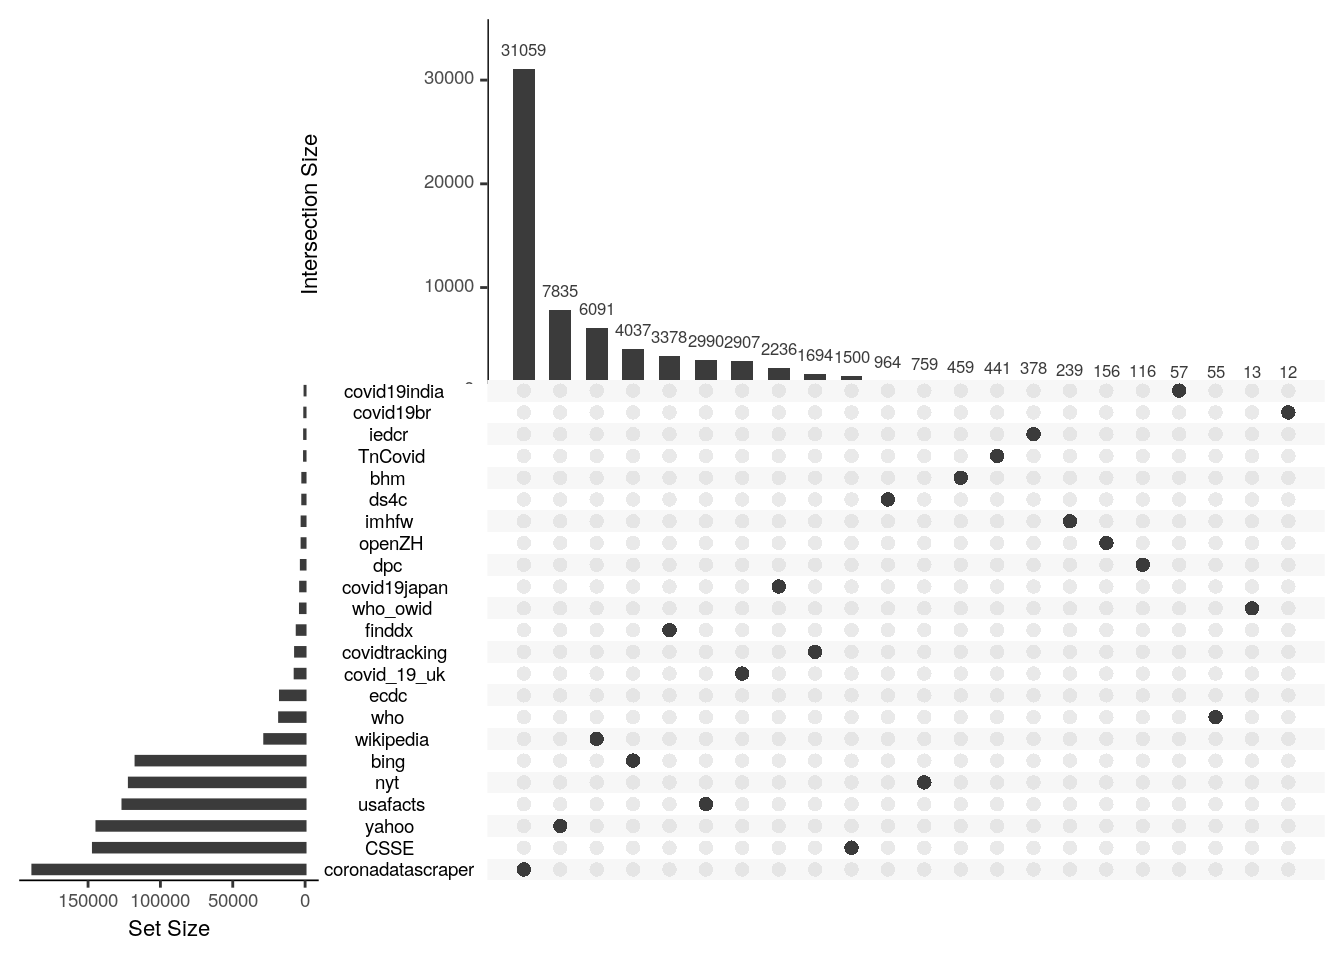
\includegraphics[width=1\linewidth]{HowToBeCarefulWithCovid19Counts_files/figure-latex/upset-1} \end{center}

\hypertarget{what-is-their-geographic-coverage}{%
\subsubsection{What is their geographic coverage?}\label{what-is-their-geographic-coverage}}

\hypertarget{country-level-data-availability}{%
\subsubsection{Country Level Data Availability}\label{country-level-data-availability}}

Despite this major effort by data producers, collectors, and aggregators, there is still major geographic variation in availability across countries. Most notably in availability of counts on number of tests performed, particularly in Central Africa.

\begin{figure}

{\centering 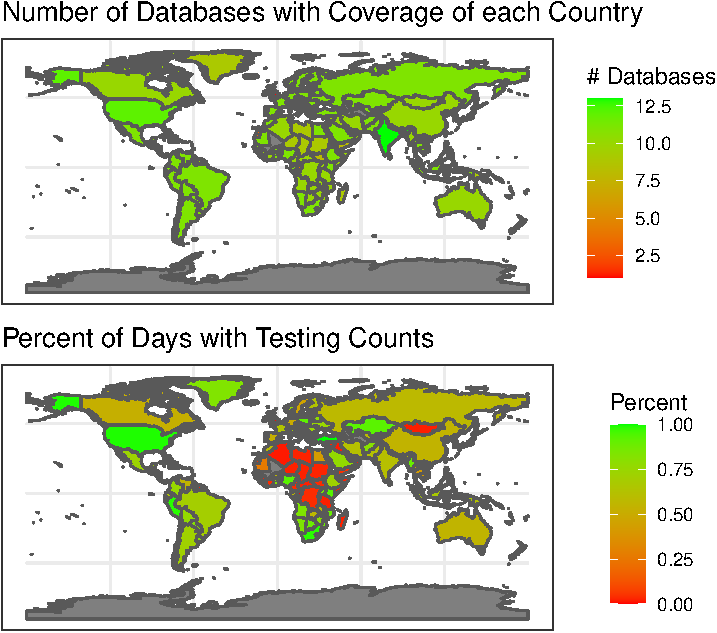
\includegraphics{HowToBeCarefulWithCovid19Counts_files/figure-latex/nice-fig2-1} 

}

\caption{Data coverage by country.}\label{fig:nice-fig2}
\end{figure}

\hypertarget{stateprovince-level-data-availability}{%
\subsubsection{State/Province Level Data Availability}\label{stateprovince-level-data-availability}}

Disparities in coverage across countries is most dramatic at the subnational level.

\begin{figure}

{\centering 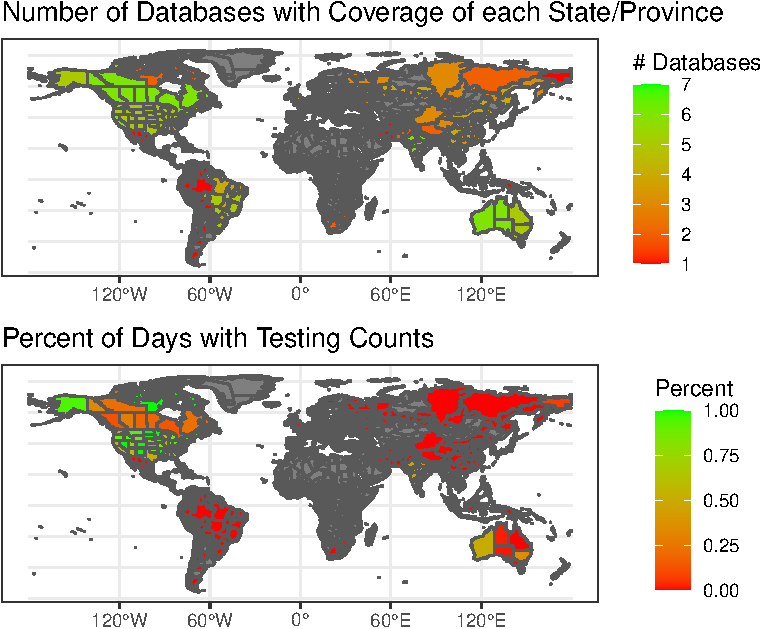
\includegraphics{HowToBeCarefulWithCovid19Counts_files/figure-latex/nice-fig3-1} 

}

\caption{Data coverage by State/Province}\label{fig:nice-fig3}
\end{figure}

\hypertarget{county-district-level-data-availability}{%
\subsection{County District Level Data Availability}\label{county-district-level-data-availability}}

This takes a long time to run so we're disabling it until the end

This takes a long time to run so we're disabling it until the end

\hypertarget{what-is-their-temporal-coverage}{%
\subsection{What is their temporal coverage?}\label{what-is-their-temporal-coverage}}

\hypertarget{coverage-across-three-countries}{%
\subsubsection{Coverage Across Three Countries}\label{coverage-across-three-countries}}

Figures x,y,z illustrate the problem of data coverage for 3 countries, China, Italy, and the U.S.

China outright refuses to release daily counts of testing. Only three databases document the beginning of the outbreak, the ECDC, the WHO, and Yahoo. On April 17, China \href{http://en.nhc.gov.cn/2020-04/17/c_79285.htm}{changed its reporting} which added 1,290 more deaths for Wuhan city only. The change is not retrospective, it shows up only a sharp discontinuity across multiple datasets.

\begin{center}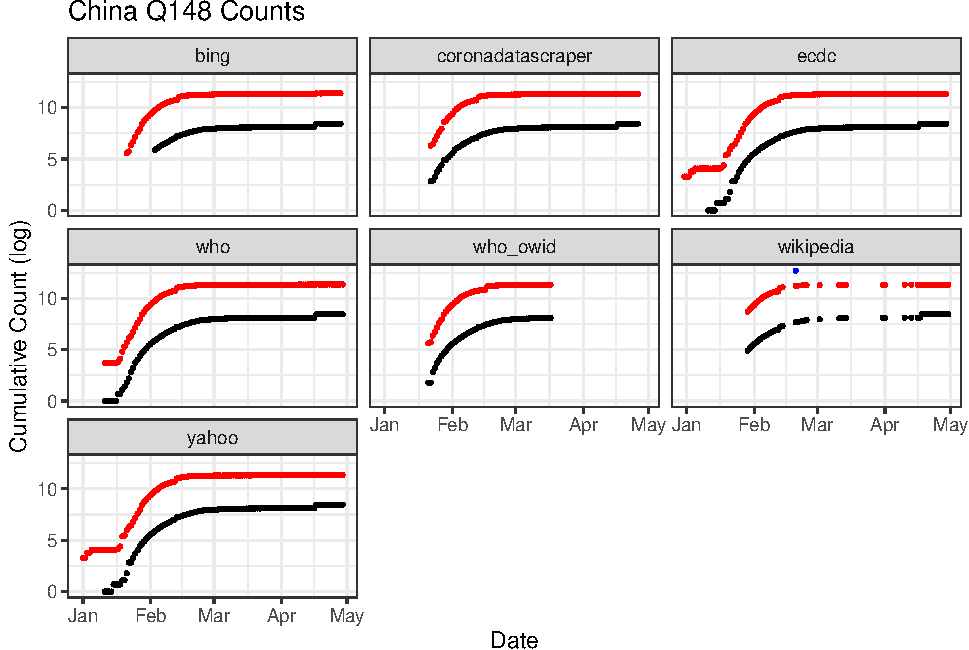
\includegraphics[width=1\linewidth]{HowToBeCarefulWithCovid19Counts_files/figure-latex/p_over_time_by_source_china1-1} \end{center}

Italy's coverage across datasets is fairly good and uniform, though there are breaks in coverage of testing for some datasets as well as variation in when each dataset starts tracking testing.

\begin{center}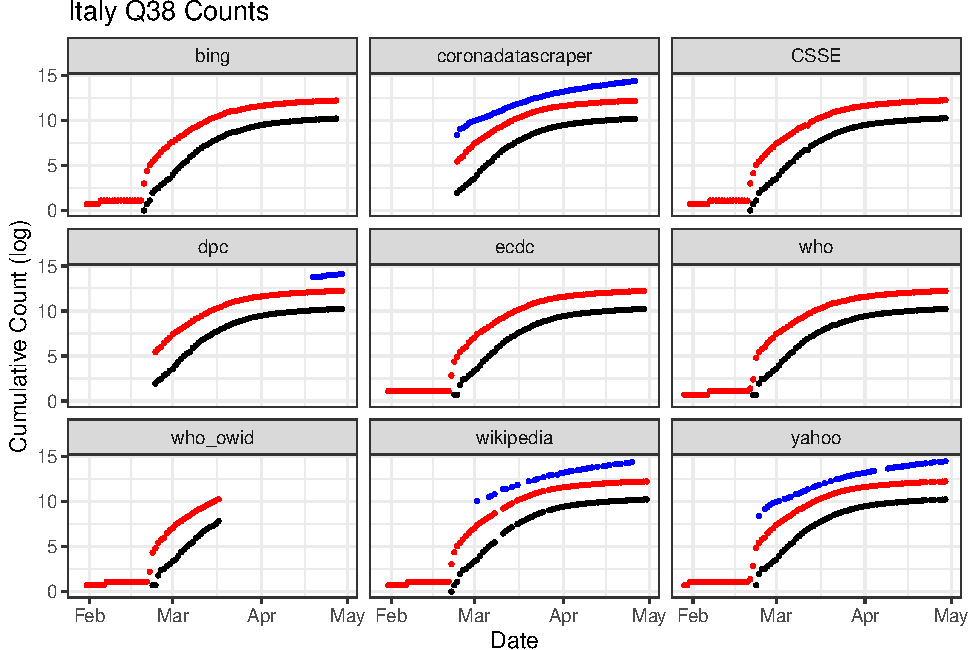
\includegraphics[width=1\linewidth]{HowToBeCarefulWithCovid19Counts_files/figure-latex/p_over_time_by_source_italy1-1} \end{center}

The U.S. has a great deal of coverage, but also a great deal of disagreement in that coverage. There is a stair step pattern in confirmed and deaths for Bing, WHO, and Wikipedia. In others reporting from day to day looks more continuous. There is also a change in reporting in late February that shows us a sharp vertical discontinuity across most datasets, though the size of the jump varies. There is also less temporal coverage of testing than is available from the caronavirus tracking project at the state level. Why those state level estiamtes aren't totaled and available at the national level is a question.

\begin{center}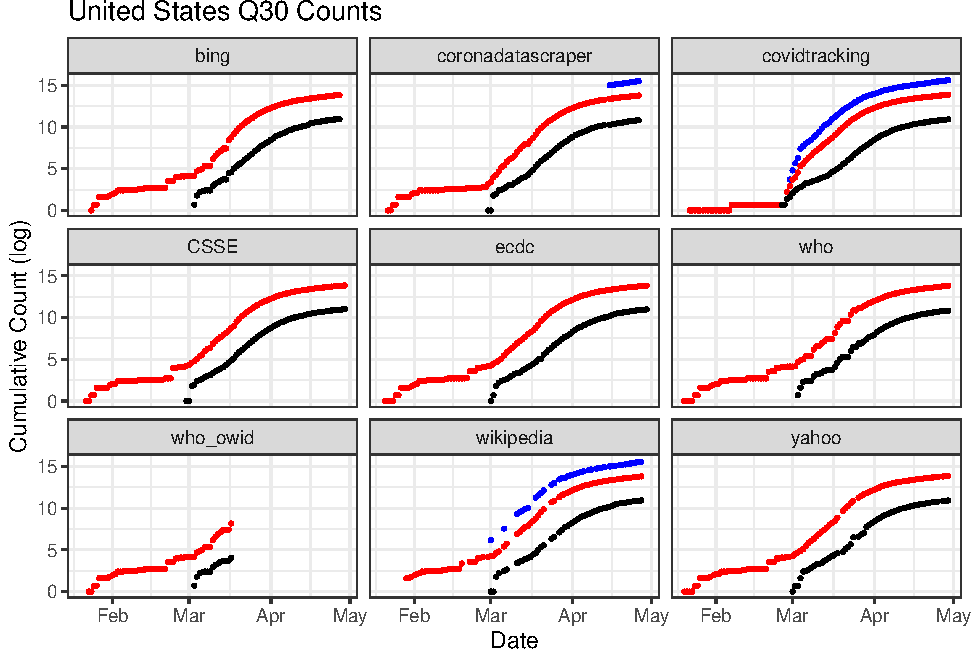
\includegraphics[width=1\linewidth]{HowToBeCarefulWithCovid19Counts_files/figure-latex/p_over_time_by_source_us1-1} \end{center}

New York has been the most heavily hit by COVID-19 in the U.S. Two sources, CornaDataScraper and the Covid Tracking Project have coverage over nearly the entire period. However, only one shows a sharp discontinuity in testing around March 10th. Digging into that disagreement more, the CTP rates New York's data release a B quality, coming from snapshots of press conferences and then switching to screenshots of New York's ``Department of Health Covid-19 Tracker'' website.

\begin{center}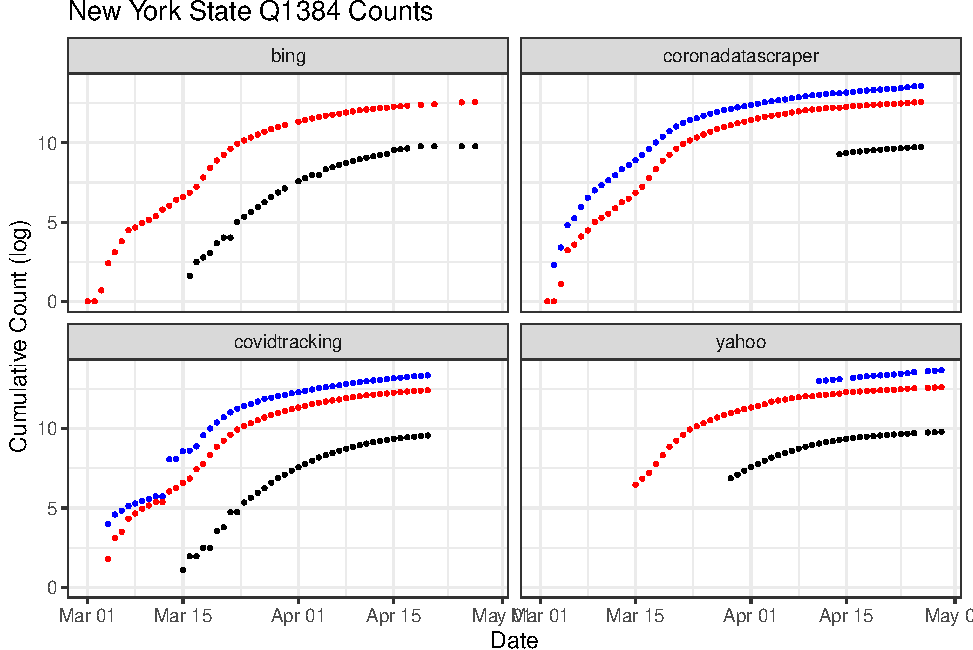
\includegraphics[width=1\linewidth]{HowToBeCarefulWithCovid19Counts_files/figure-latex/p_over_time_by_source_new_york_state1-1} \end{center}

\begin{center}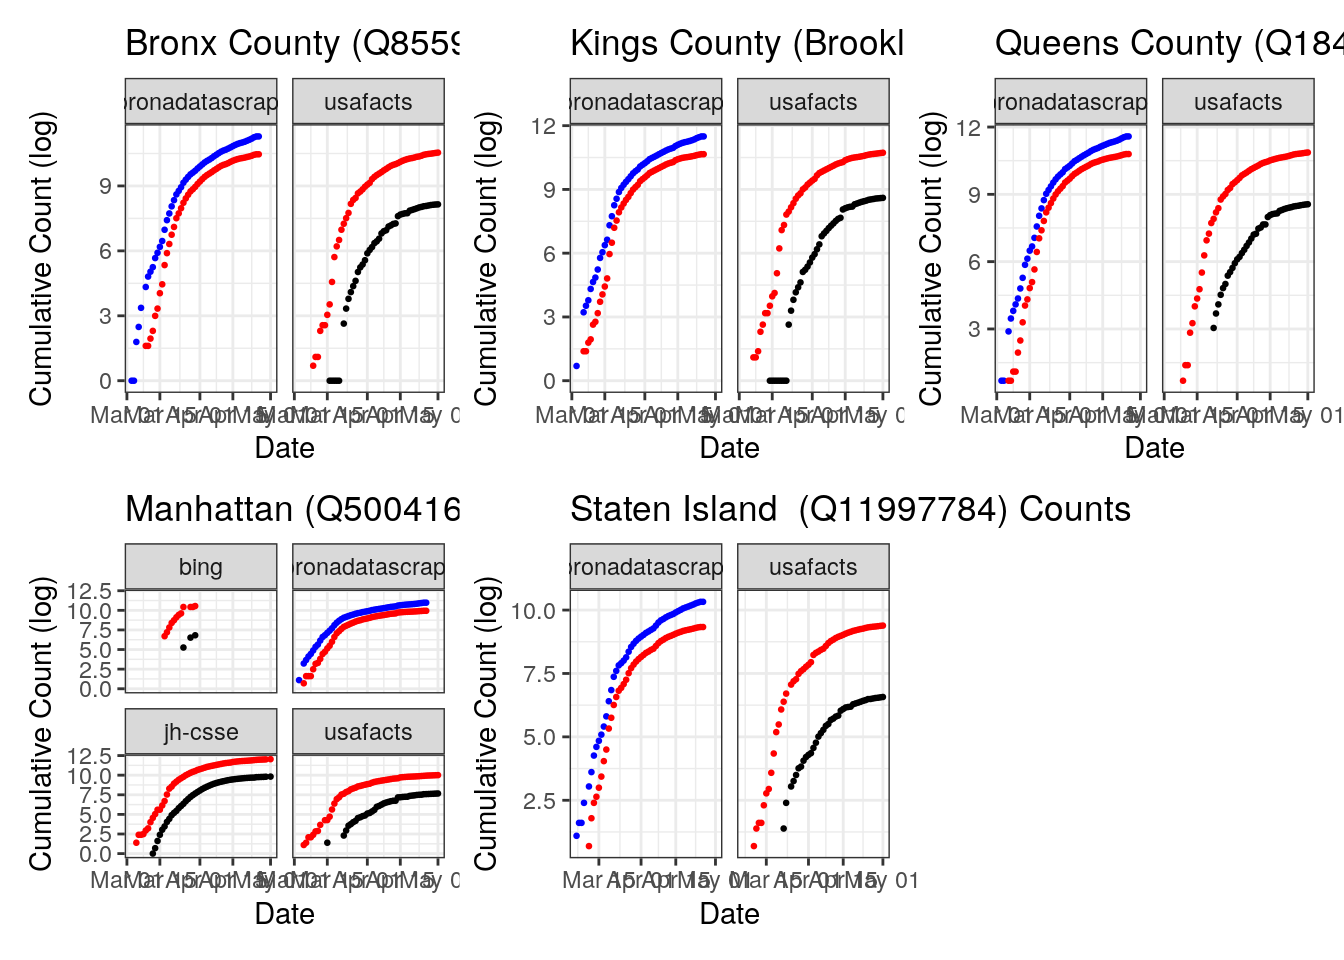
\includegraphics[width=1\linewidth]{HowToBeCarefulWithCovid19Counts_files/figure-latex/unnamed-chunk-27-1} \end{center}

\hypertarget{where-and-how-do-they-disagree}{%
\subsection{Where and How do they Disagree?}\label{where-and-how-do-they-disagree}}

\hypertarget{influenza-survailance}{%
\section{Influenza Survailance}\label{influenza-survailance}}

This is the main page for links on weekly mortality data
\url{https://www.cdc.gov/nchs/nvss/vsrr/covid_weekly/}
``The National Center for Health Statistics (NCHS) uses incoming data from death certificates to produce provisional COVID-19 death counts. These include deaths occurring within the 50 states and the District of Columbia. COVID-19 deaths are identified using a new ICD--10 code. When COVID-19 is reported as a cause of death -- or when it is listed as a ``probable'' or ``presumed'' cause --- the death is coded as U07.1. This can include cases with or without laboratory confirmation."

``Provisional COVID-19 Death Counts by Week Ending Date and State''
\url{https://data.cdc.gov/NCHS/Provisional-COVID-19-Death-Counts-by-Week-Ending-D/r8kw-7aab}

There is technically raw data but the csv is aweful
Gives you age stratified number tested and the percent positive
\url{https://www.cdc.gov/coronavirus/2019-ncov/covid-data/covidview/05082020/csv/public-health-lab.csv}
\url{https://data.cdc.gov/api/views/r8kw-7aab/rows.csv?accessType=DOWNLOAD}

For now I might have to download this all by hand

CDC COVID-NET Weekly Report: COVID-19-Associated
Hospitalizations Application Quick Reference Guide
\url{https://gis.cdc.gov/grasp/COVIDNet/Documents/316429-A_FS_COVID-NET\%20Helpquick\%20Reference\%20Guide_FINAL.pdf}
``Data gathered are used to estimate agespecific hospitalization rates on a weekly basis and describe characteristics of persons hospitalized with COVID-19. Laboratory confirmation is dependent on clinicianordered SARS-CoV-2 testing. Therefore, the rates provided are likely to be underestimated as COVID-19-associated hospitalizations can be missed due to test availability and provider or facility testing practices.''

``Mortality Surveillance
The National Center for Health Statistics (NCHS) collects death certificate data from vital statistics offices for all deaths occurring in the United States. Based on death certificate data available on May 7, 2020, 10.6\% of all deaths occurring during the week ending May 2, 2020 (week 18) were due to pneumonia, influenza or COVID-19 (PIC). This is the third week of a stable or declining percentage of deaths due to PIC;''

\url{https://catalog.data.gov/dataset/deaths-from-pneumonia-and-influenza-pi-and-all-deaths-by-state-and-region-national-center-}

\url{https://www.cdc.gov/nchs/nvss/covid-19.htm}
Updated daily, Monday--Friday

Provisional Death Counts for Coronavirus Disease (COVID-19)

Tabulated data on provisional death counts for COVID-19, by week, jurisdiction, and age in the U.S.

Updated weekly

Weekly State-Specific Data Updates by Select Demographic and Geographic Characteristics

Tabulated data on provisional COVID-19 deaths by race and Hispanic origin

Updated weekly

Excess Deaths Associated with COVID-19

Visualizations of estimates of excess deaths related to the COVID-19 pandemic

\hypertarget{motaility-survailance}{%
\section{Motaility Survailance}\label{motaility-survailance}}

\hypertarget{covid-19-inference}{%
\chapter{COVID-19 Inference}\label{covid-19-inference}}

In this chapter I will introduce parameters we wish to infer about COVID-19 spread and a modeling approach that can recover them from the observable introduced in the last chapter. I will add components to the model one piece at a time so that their function and impact on inference are clear.

\hypertarget{confirmed-cases}{%
\section{Confirmed Cases}\label{confirmed-cases}}

\begin{center}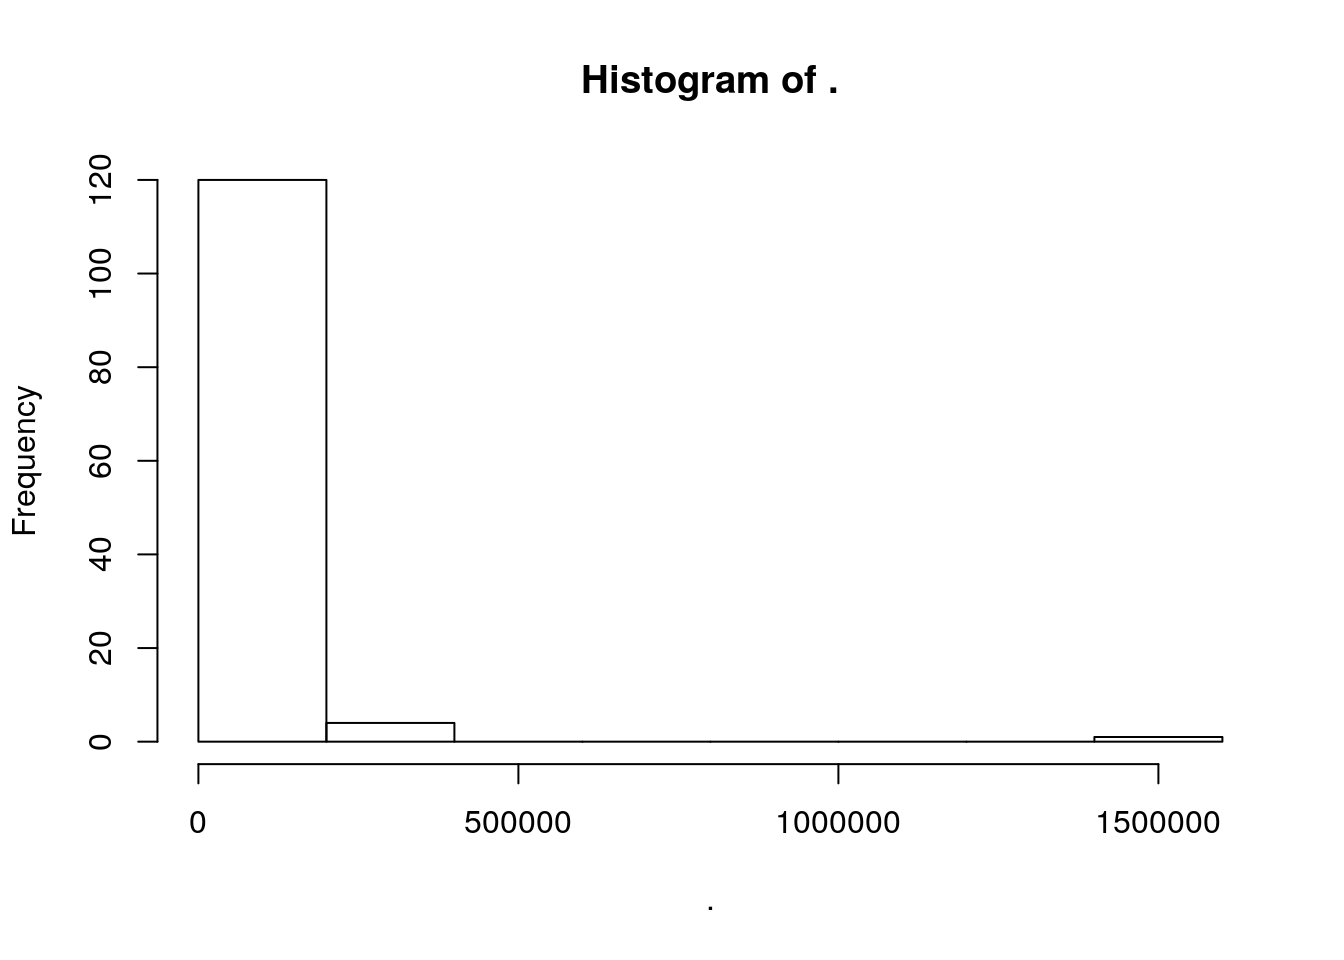
\includegraphics[width=1\linewidth]{HowToBeCarefulWithCovid19Counts_files/figure-latex/unnamed-chunk-37-1} \end{center}

\begin{center}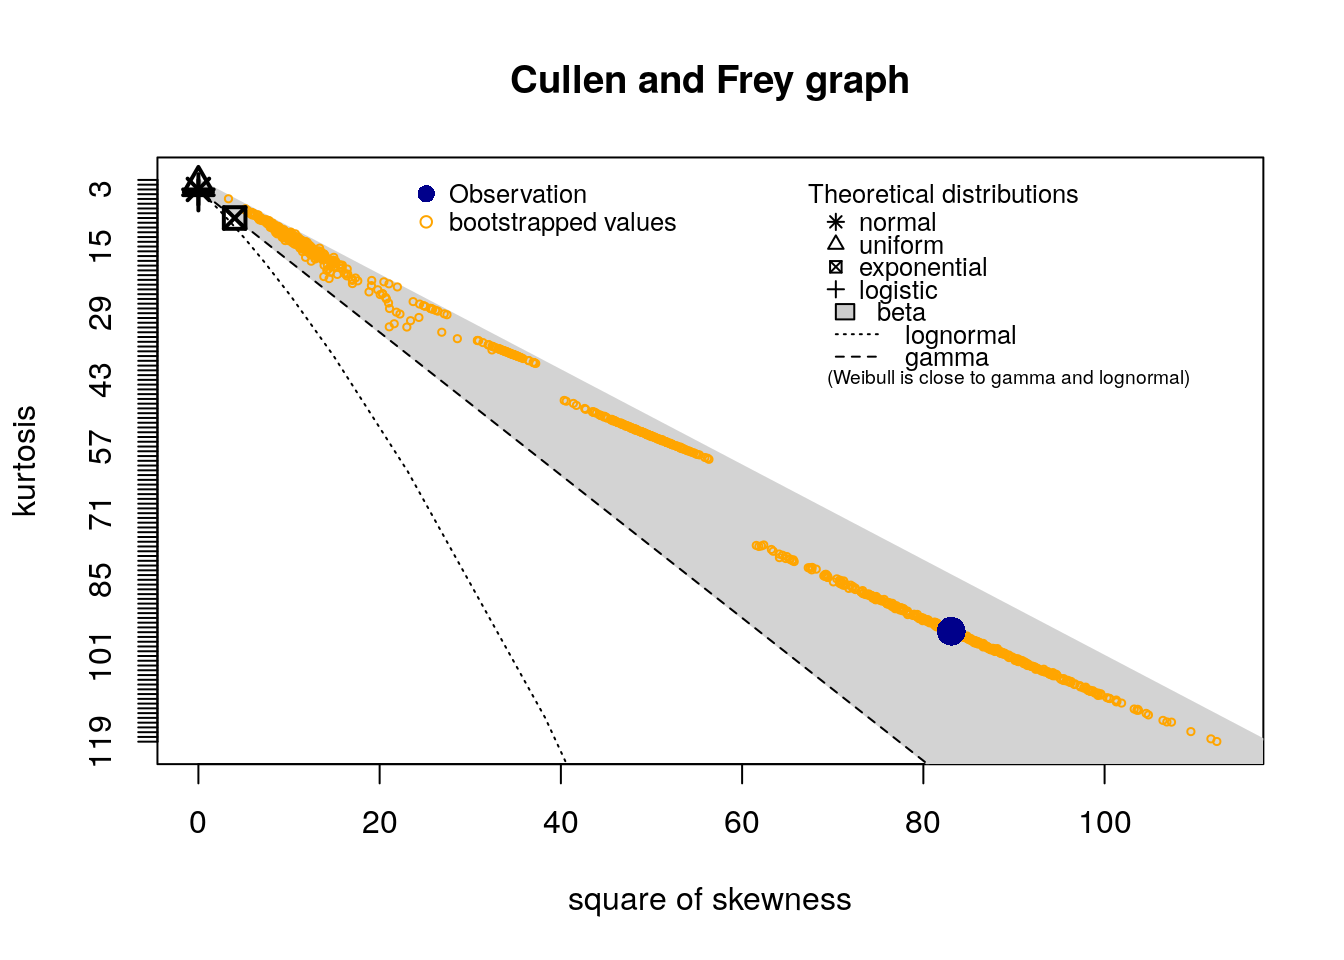
\includegraphics[width=1\linewidth]{HowToBeCarefulWithCovid19Counts_files/figure-latex/unnamed-chunk-37-2} \end{center}

\begin{center}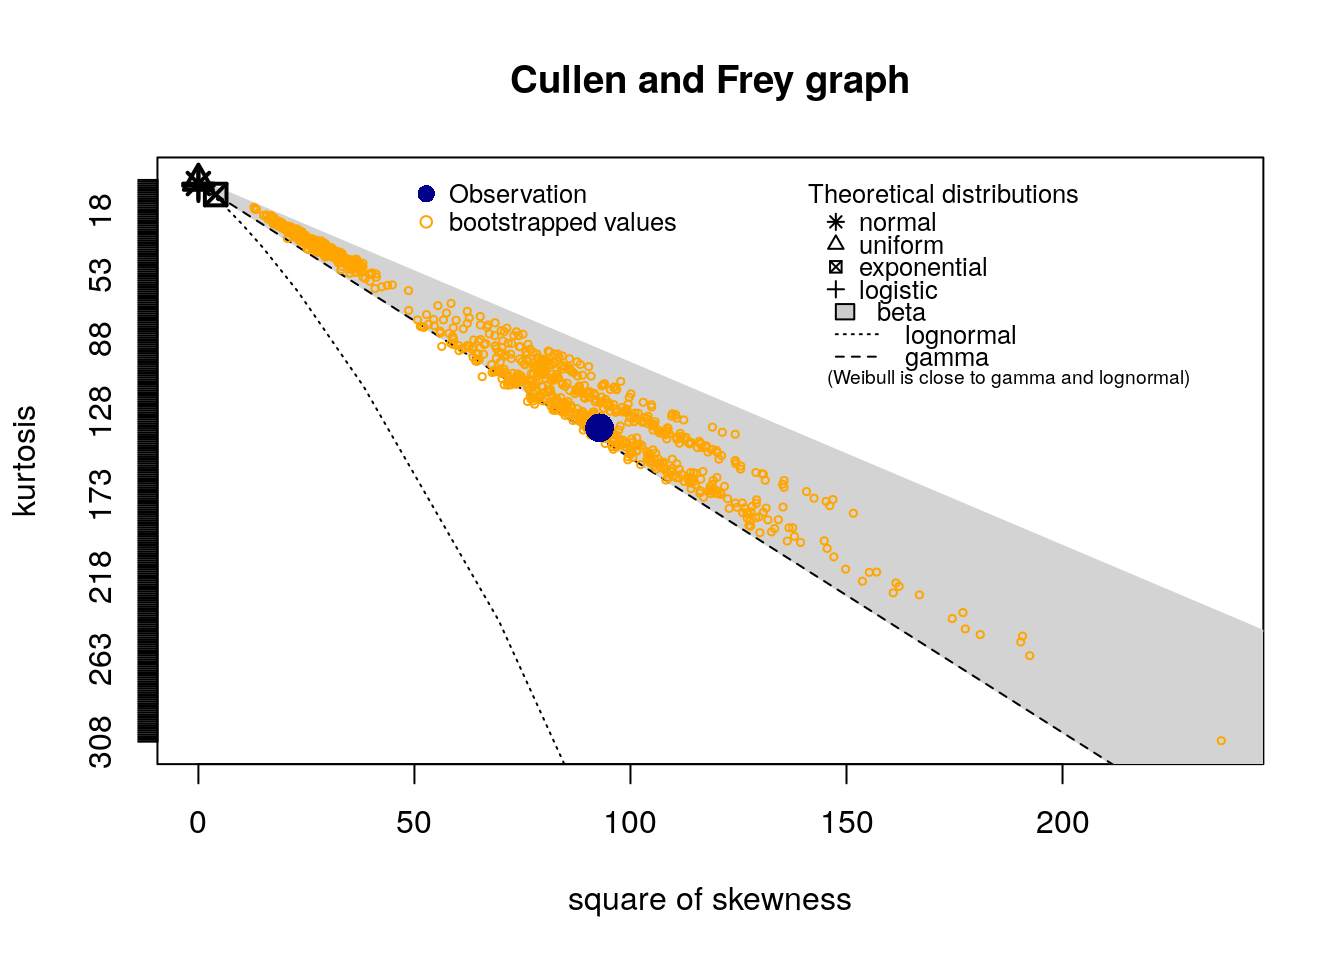
\includegraphics[width=1\linewidth]{HowToBeCarefulWithCovid19Counts_files/figure-latex/unnamed-chunk-37-3} \end{center}

\begin{center}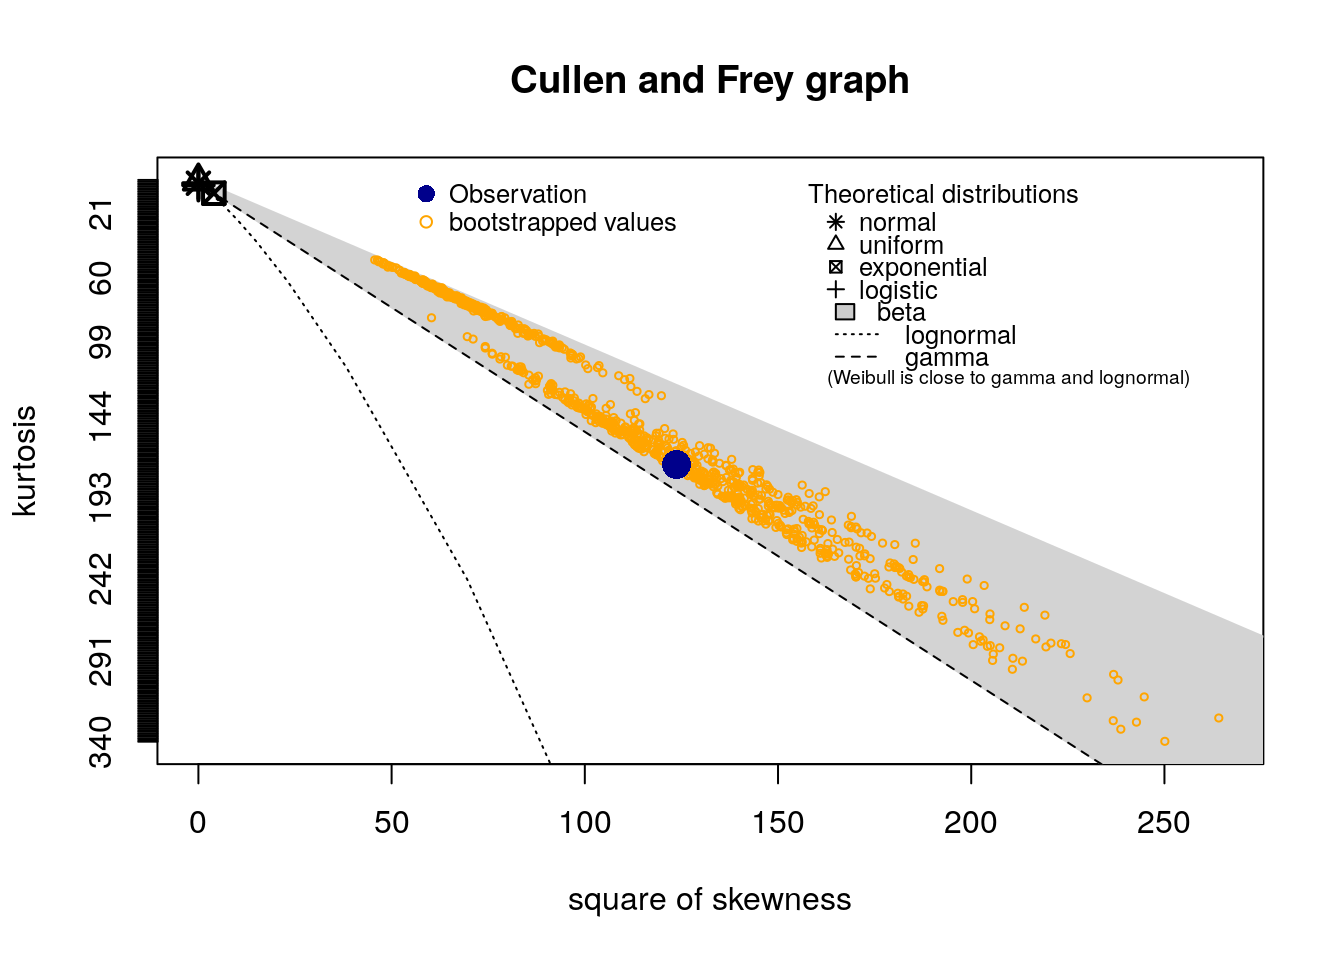
\includegraphics[width=1\linewidth]{HowToBeCarefulWithCovid19Counts_files/figure-latex/unnamed-chunk-37-4} \end{center}

\begin{center}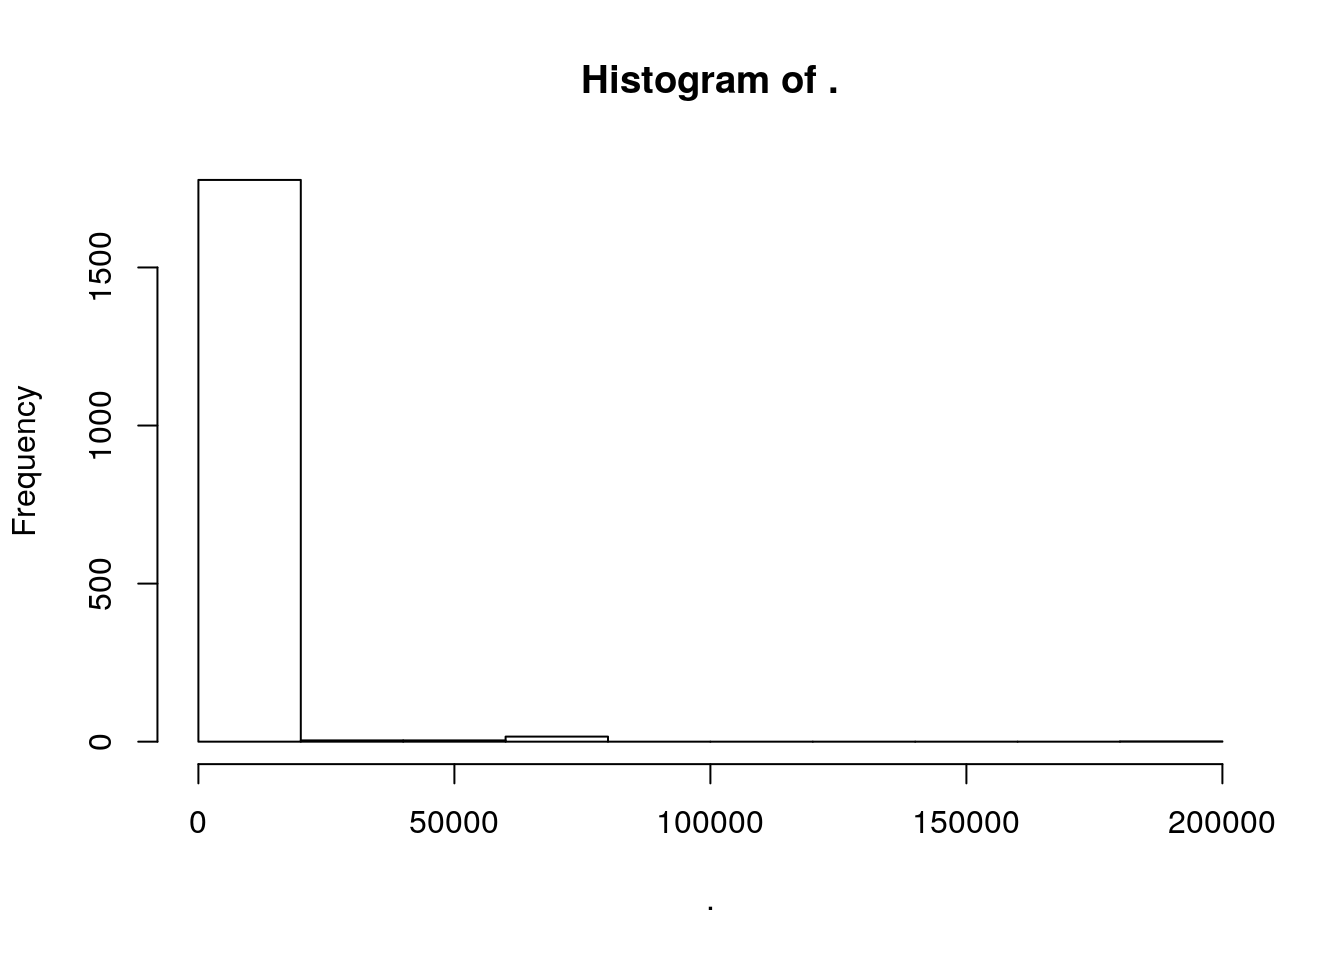
\includegraphics[width=1\linewidth]{HowToBeCarefulWithCovid19Counts_files/figure-latex/unnamed-chunk-37-5} \end{center}

\hypertarget{confirmed-case-fatality-rate-ccfr}{%
\section{Confirmed Case Fatality Rate (CCFR)}\label{confirmed-case-fatality-rate-ccfr}}

One parameter we can estimate directly from the data is the ratio of reported COVID-19 fatalities to the reported COVID-19 cases in an area. This should not be confused with the Case Fatality Rate (CFR) or the Infection Fatality Rate (IFR) which I discuss later. The CCFR is bounded between 0 and 1.

\(Confirmed Case Fataility Rate = \frac{ConfirmedCovid19Fatailities}{ConfirmedCovid19Cases}\)

\begin{center}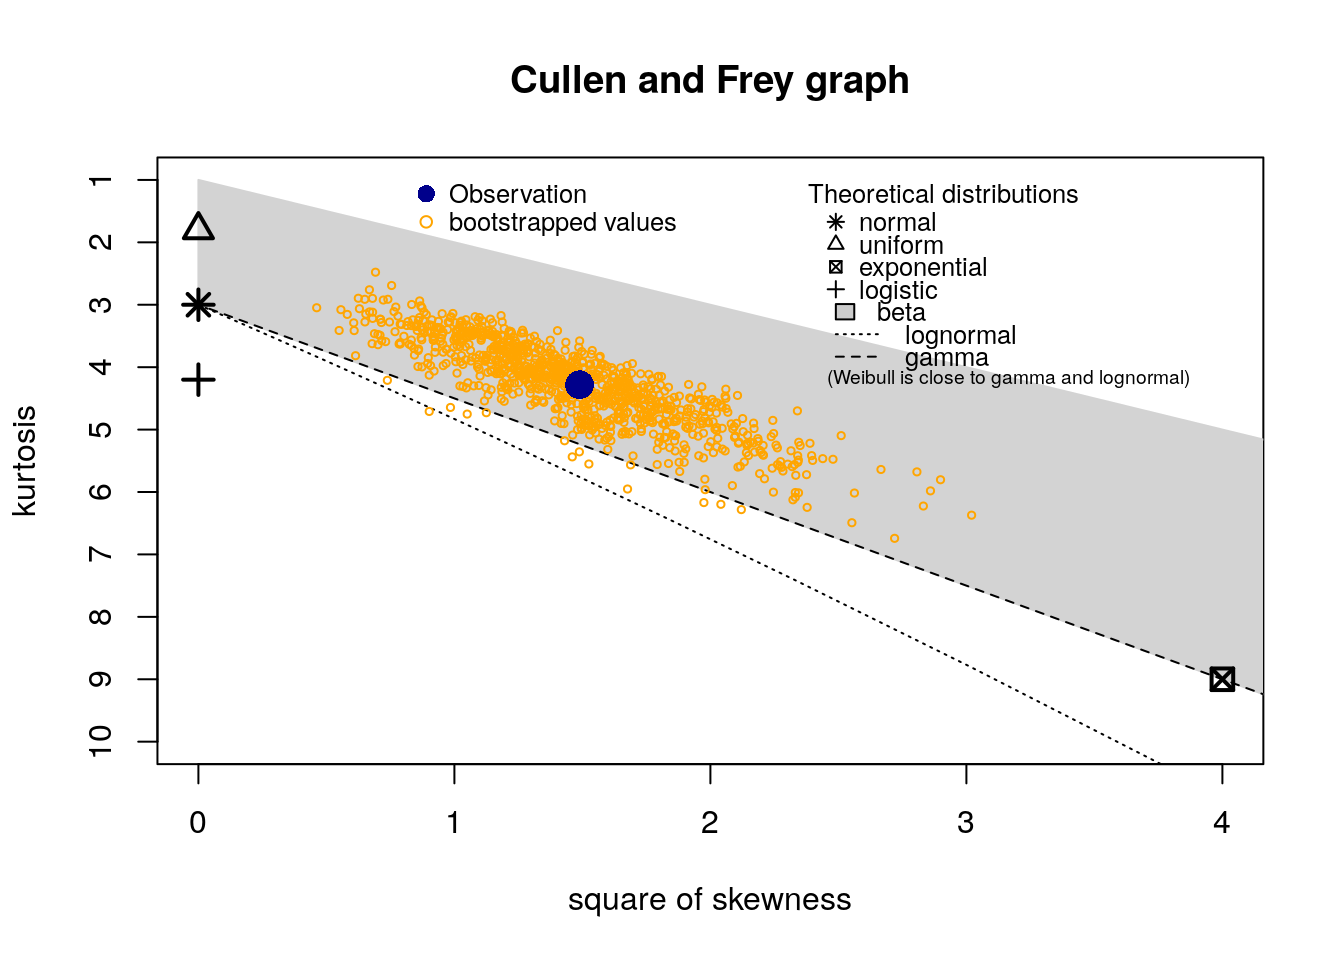
\includegraphics[width=1\linewidth]{HowToBeCarefulWithCovid19Counts_files/figure-latex/unnamed-chunk-38-1} \end{center}

\begin{center}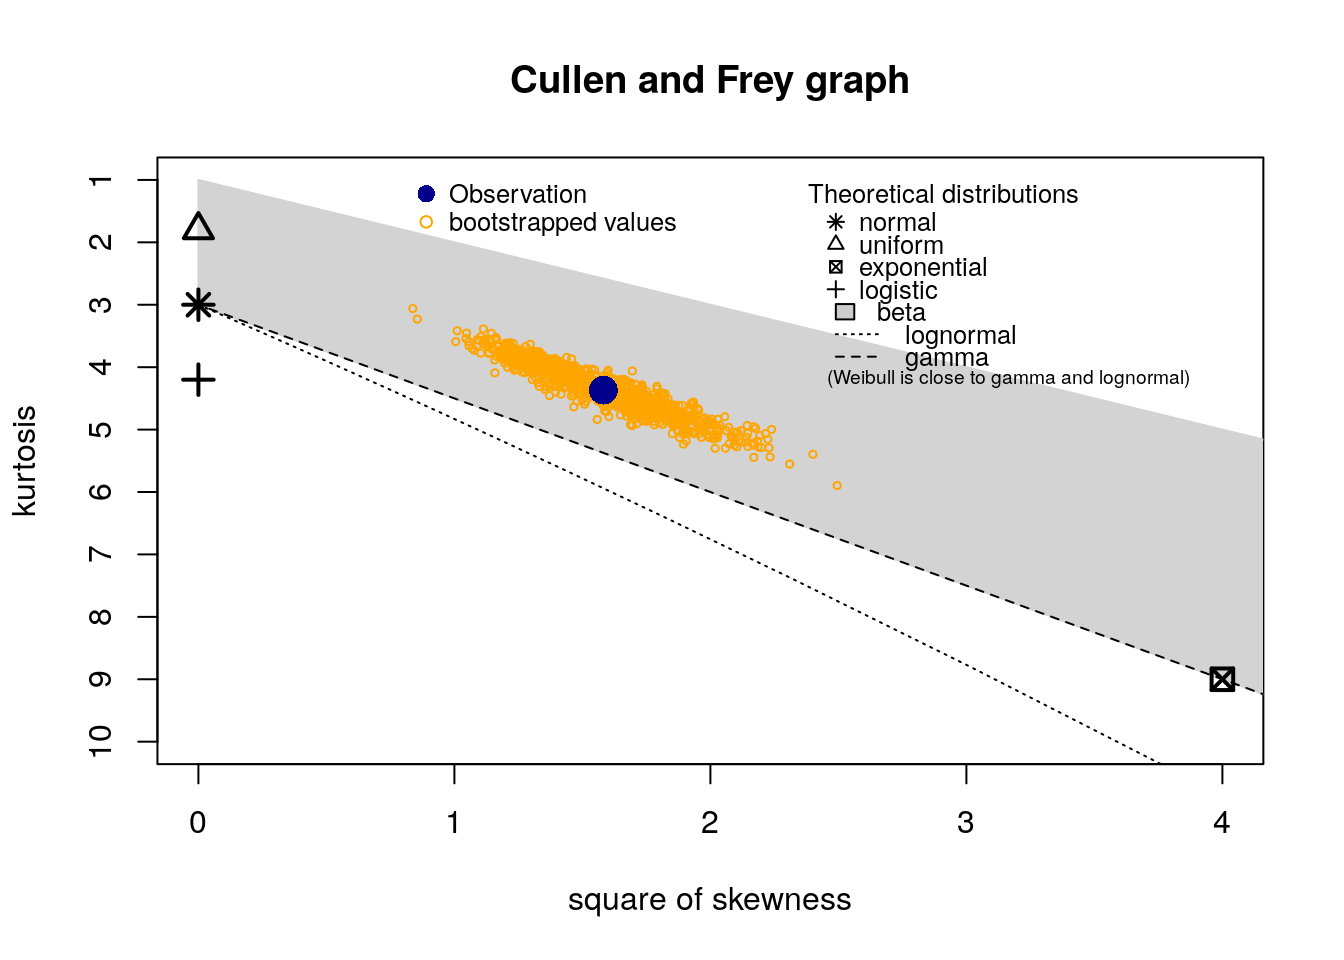
\includegraphics[width=1\linewidth]{HowToBeCarefulWithCovid19Counts_files/figure-latex/unnamed-chunk-38-2} \end{center}

\begin{center}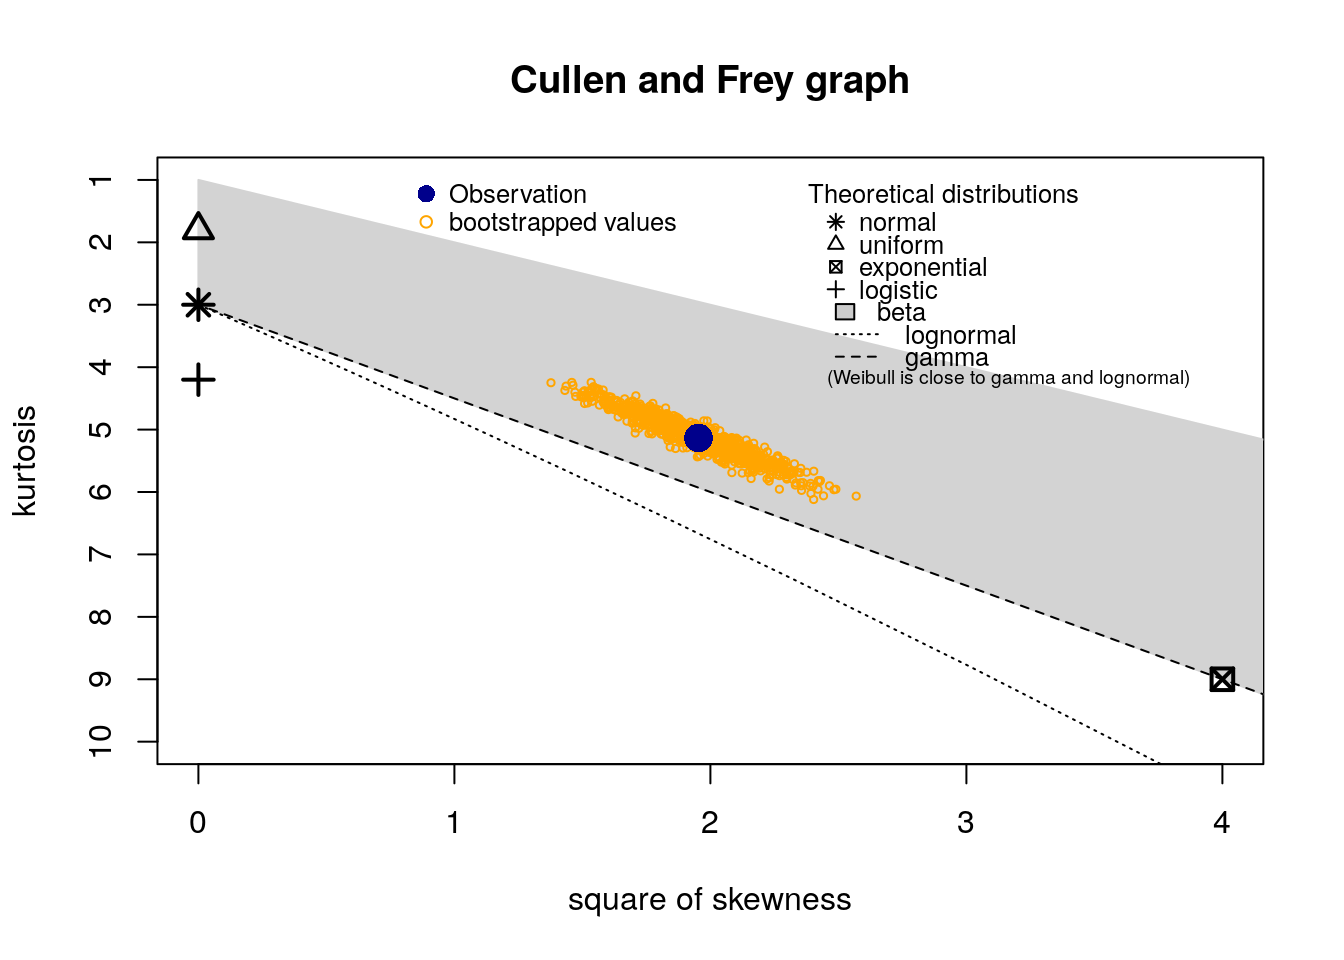
\includegraphics[width=1\linewidth]{HowToBeCarefulWithCovid19Counts_files/figure-latex/unnamed-chunk-38-3} \end{center}

\begin{center}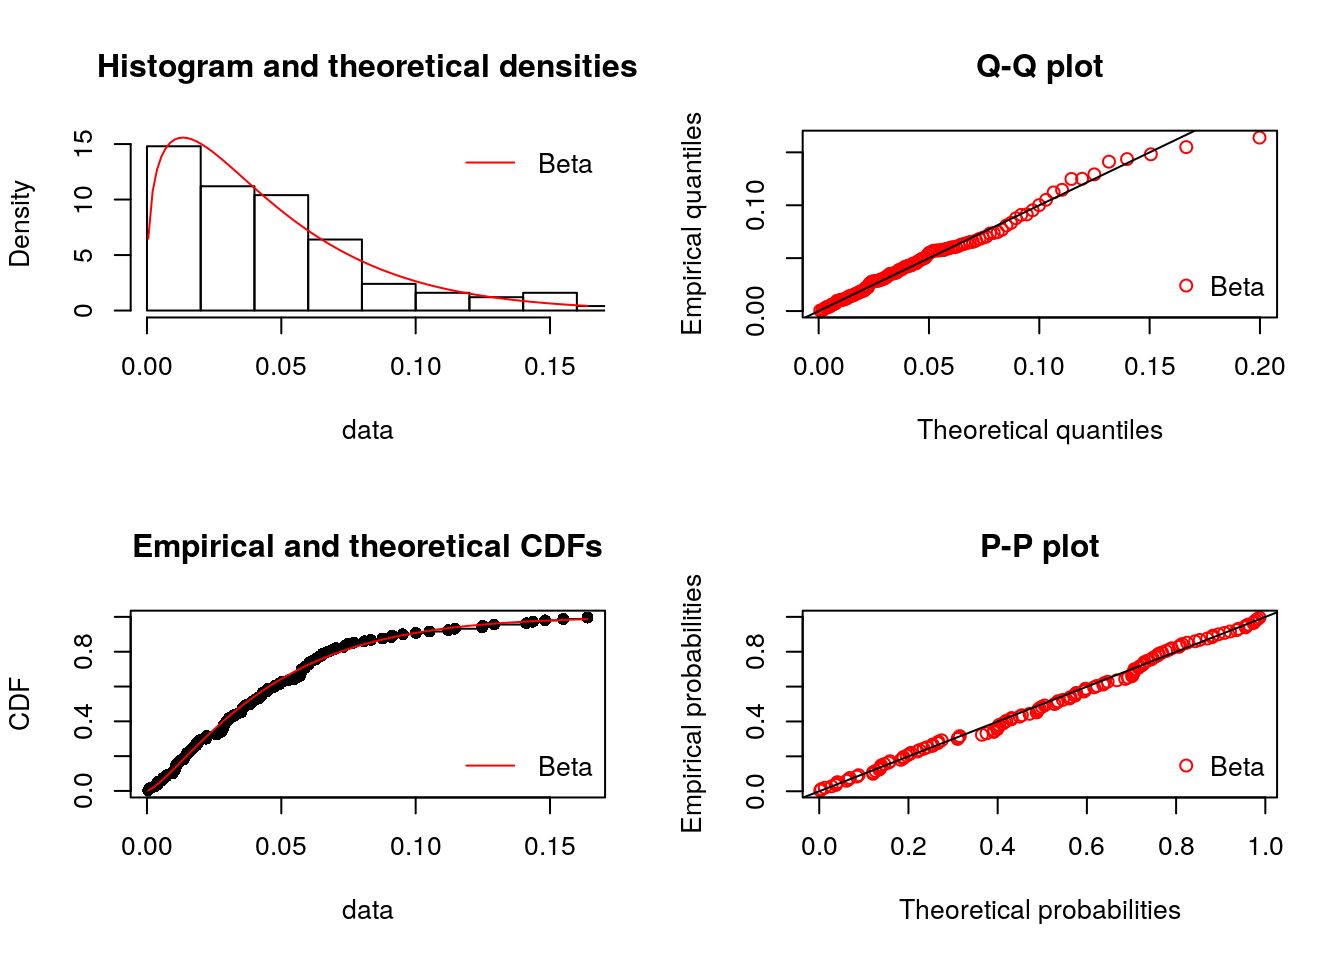
\includegraphics[width=1\linewidth]{HowToBeCarefulWithCovid19Counts_files/figure-latex/unnamed-chunk-38-4} \end{center}

\begin{center}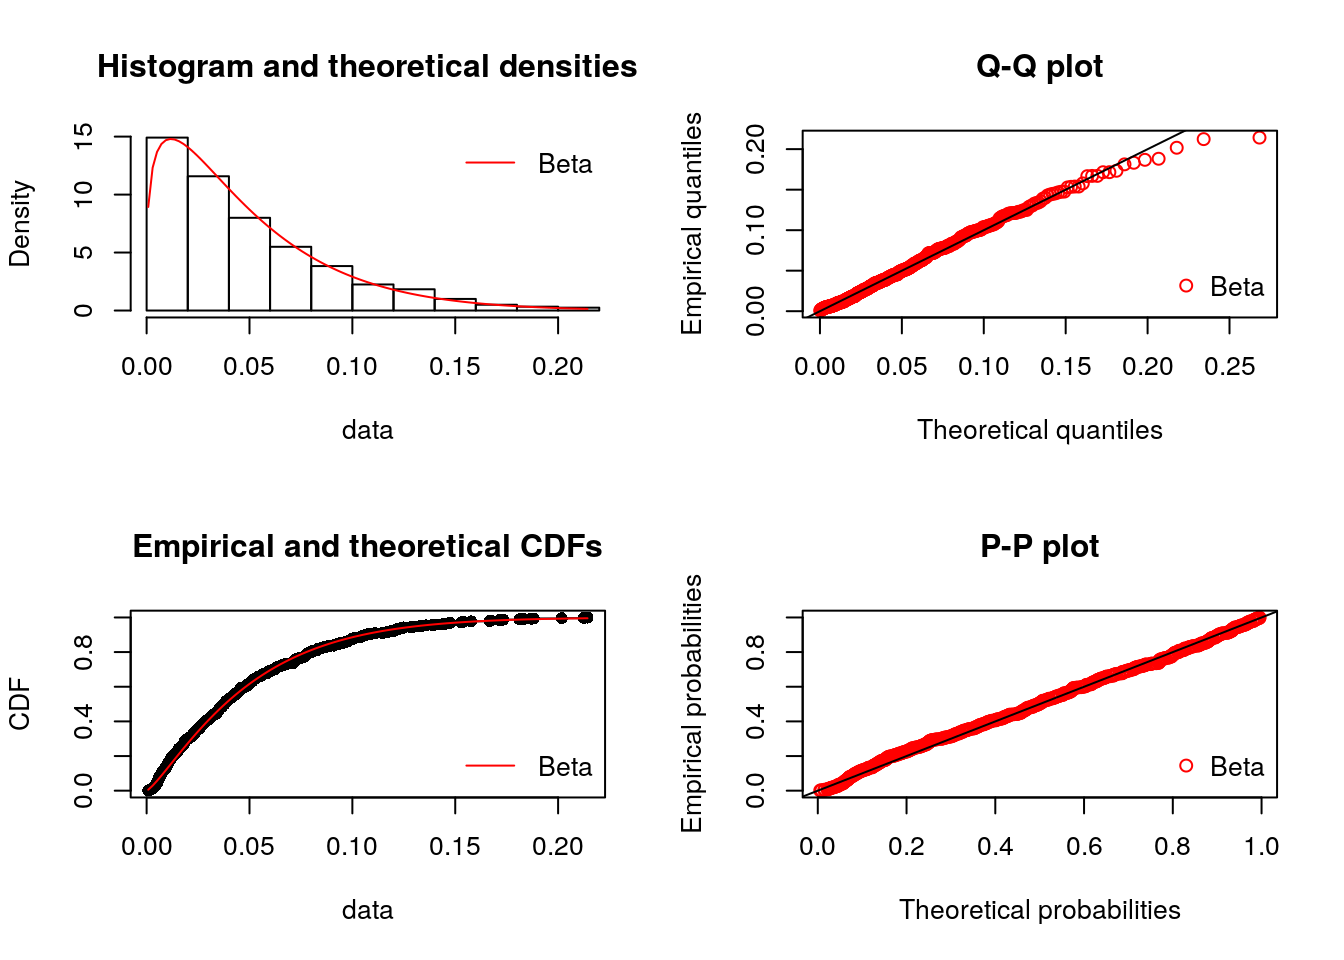
\includegraphics[width=1\linewidth]{HowToBeCarefulWithCovid19Counts_files/figure-latex/unnamed-chunk-38-5} \end{center}

\begin{center}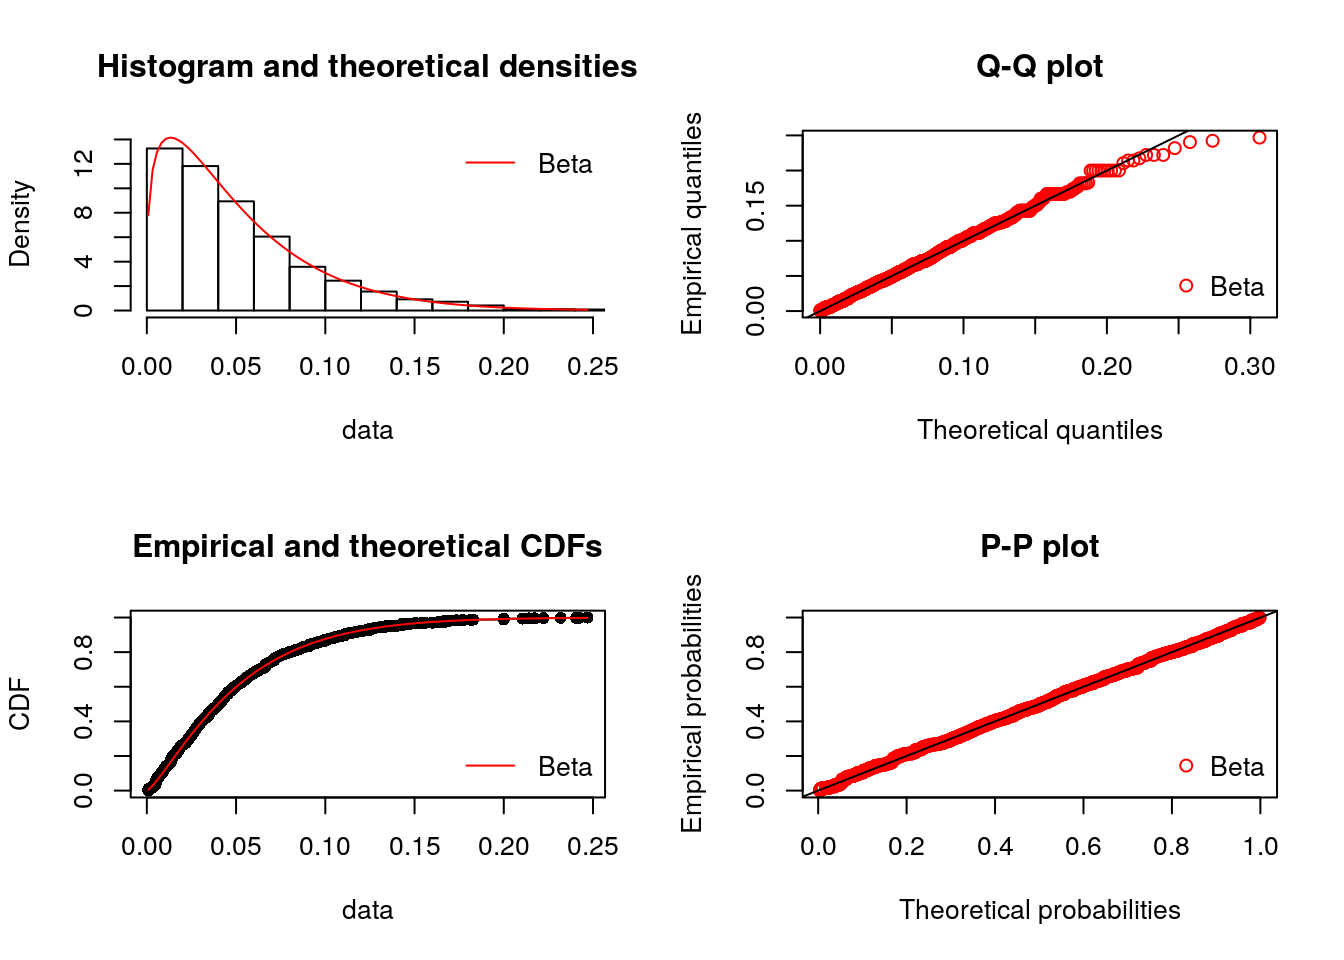
\includegraphics[width=1\linewidth]{HowToBeCarefulWithCovid19Counts_files/figure-latex/unnamed-chunk-38-6} \end{center}

\(CFR=0.07 = \frac{}{}\)

\begin{center}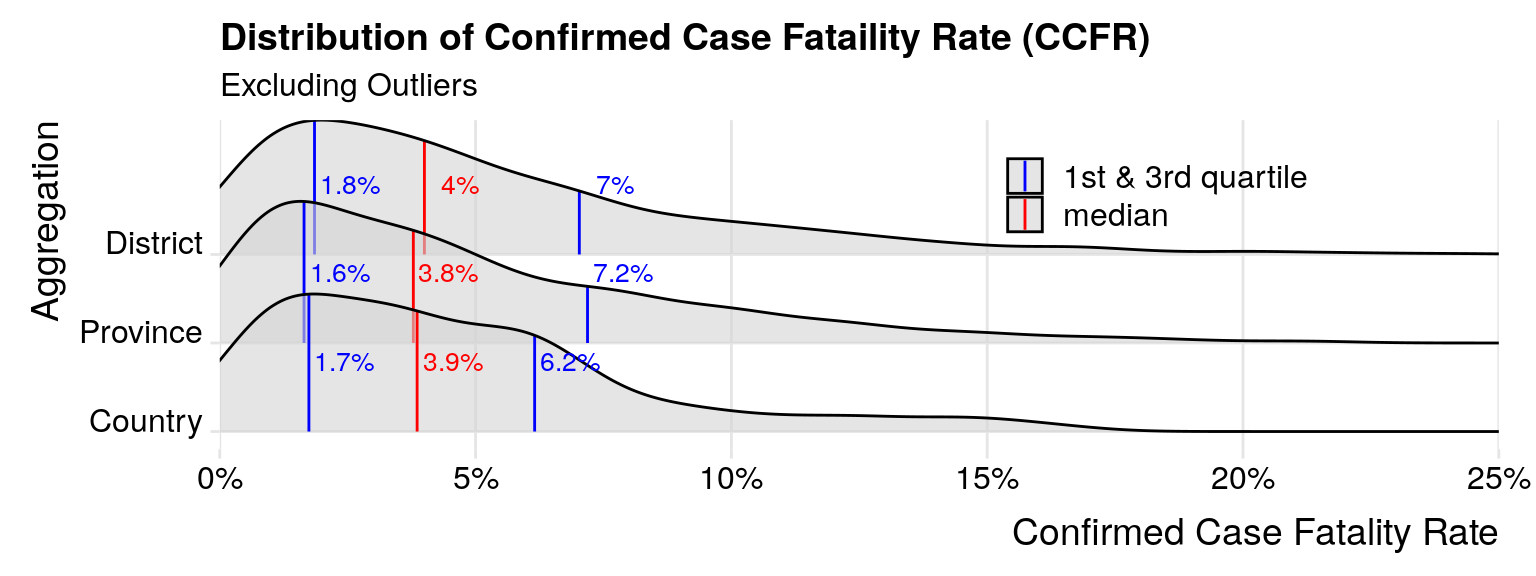
\includegraphics[width=1\linewidth]{HowToBeCarefulWithCovid19Counts_files/figure-latex/unnamed-chunk-40-1} \end{center}

\hypertarget{tests}{%
\section{Tests}\label{tests}}

\hypertarget{tested-people-versus-tested-samples}{%
\section{Tested People versus Tested Samples}\label{tested-people-versus-tested-samples}}

\hypertarget{interpolate-within-observed}{%
\section{Interpolate Within Observed}\label{interpolate-within-observed}}

\hypertarget{interplate-prior-to-observed}{%
\section{Interplate Prior to Observed}\label{interplate-prior-to-observed}}

\hypertarget{interpolate-subnationally}{%
\section{Interpolate Subnationally}\label{interpolate-subnationally}}

\hypertarget{explaining-variation-in-testing}{%
\section{Explaining Variation in Testing}\label{explaining-variation-in-testing}}

South Korea

Vietnam
\url{https://www.reuters.com/article/us-health-coronavirus-vietnam-fight-insi-idUSKBN22B34H}

\hypertarget{covid-19-causal-inference}{%
\chapter{COVID-19 Causal-Inference}\label{covid-19-causal-inference}}

\hypertarget{covid-19-prediction}{%
\chapter{COVID-19 Prediction}\label{covid-19-prediction}}

\hypertarget{conclusion}{%
\chapter{Conclusion}\label{conclusion}}

  \bibliography{My Library.bib,packages.bib}

\end{document}
